\chapter{Практические задания}

\section*{Задание 1. Составить диаграмму вычисления следующих выражений:}

\begin{figure}[h!]
	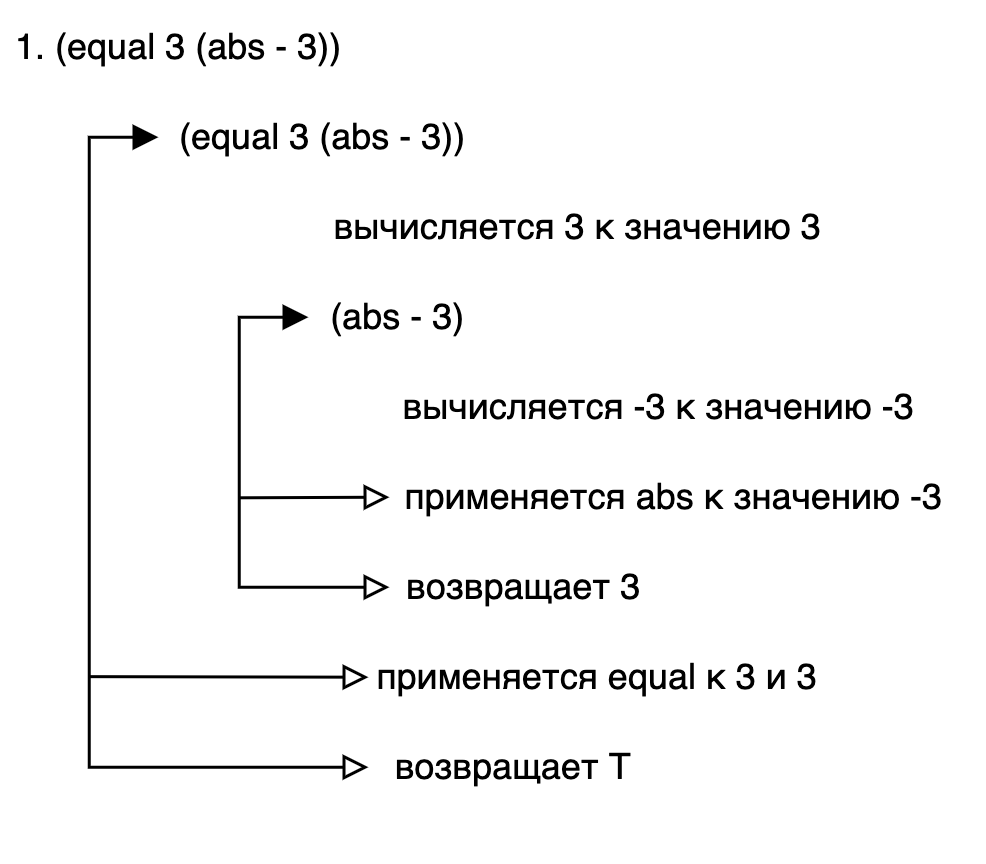
\includegraphics[scale=0.6,left]{task1.1}
\end{figure}

\begin{figure}[h!]
	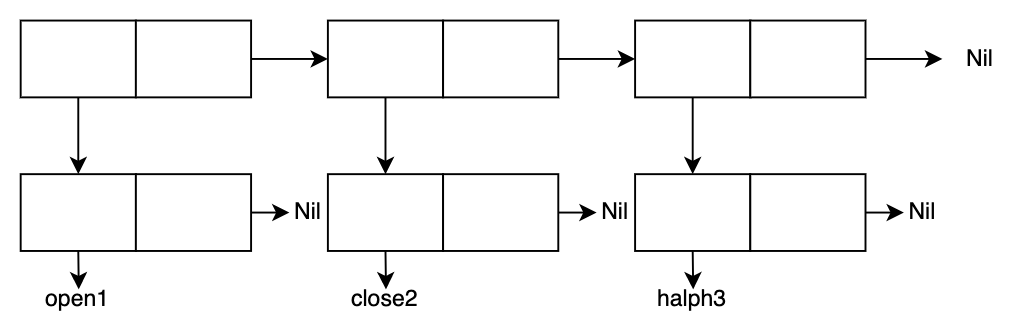
\includegraphics[scale=0.6,left]{task1.2}
\end{figure}

\begin{figure}[h!]
	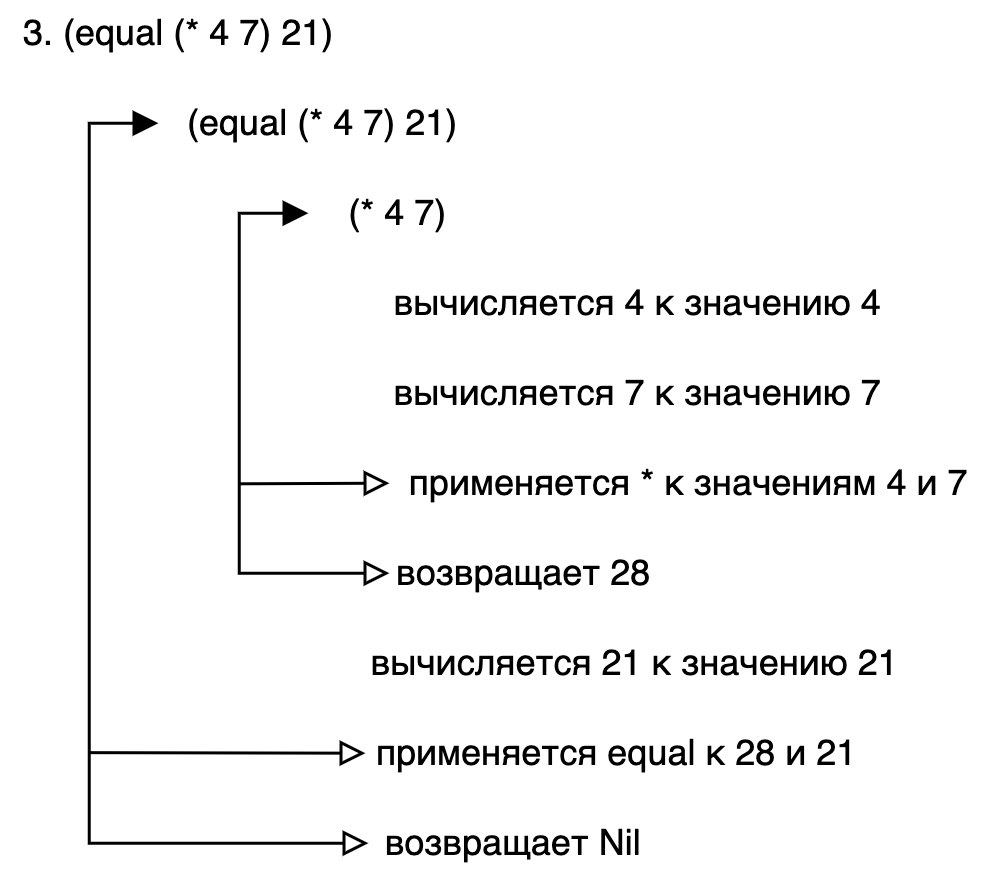
\includegraphics[scale=0.6,left]{task1.3}
\end{figure}

\begin{figure}[h!]
	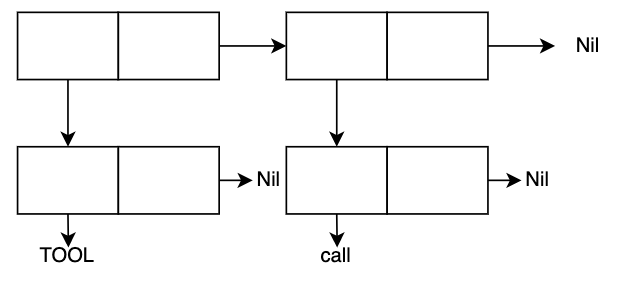
\includegraphics[scale=0.6,left]{task1.4}
\end{figure}

\begin{figure}[h!]
	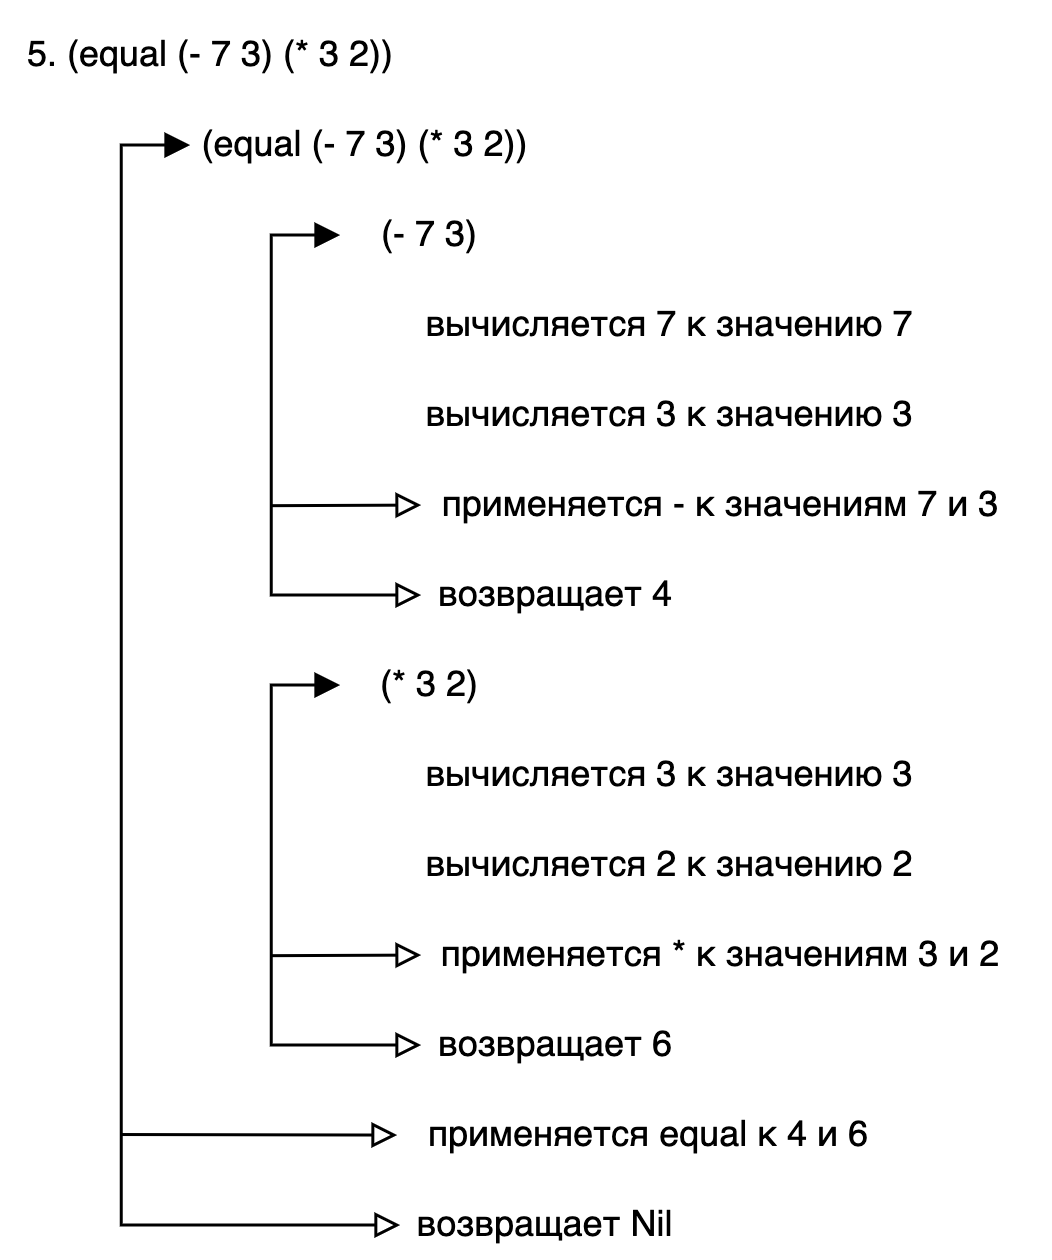
\includegraphics[scale=0.5,left]{task1.5}
\end{figure}

\begin{figure}[h!]
	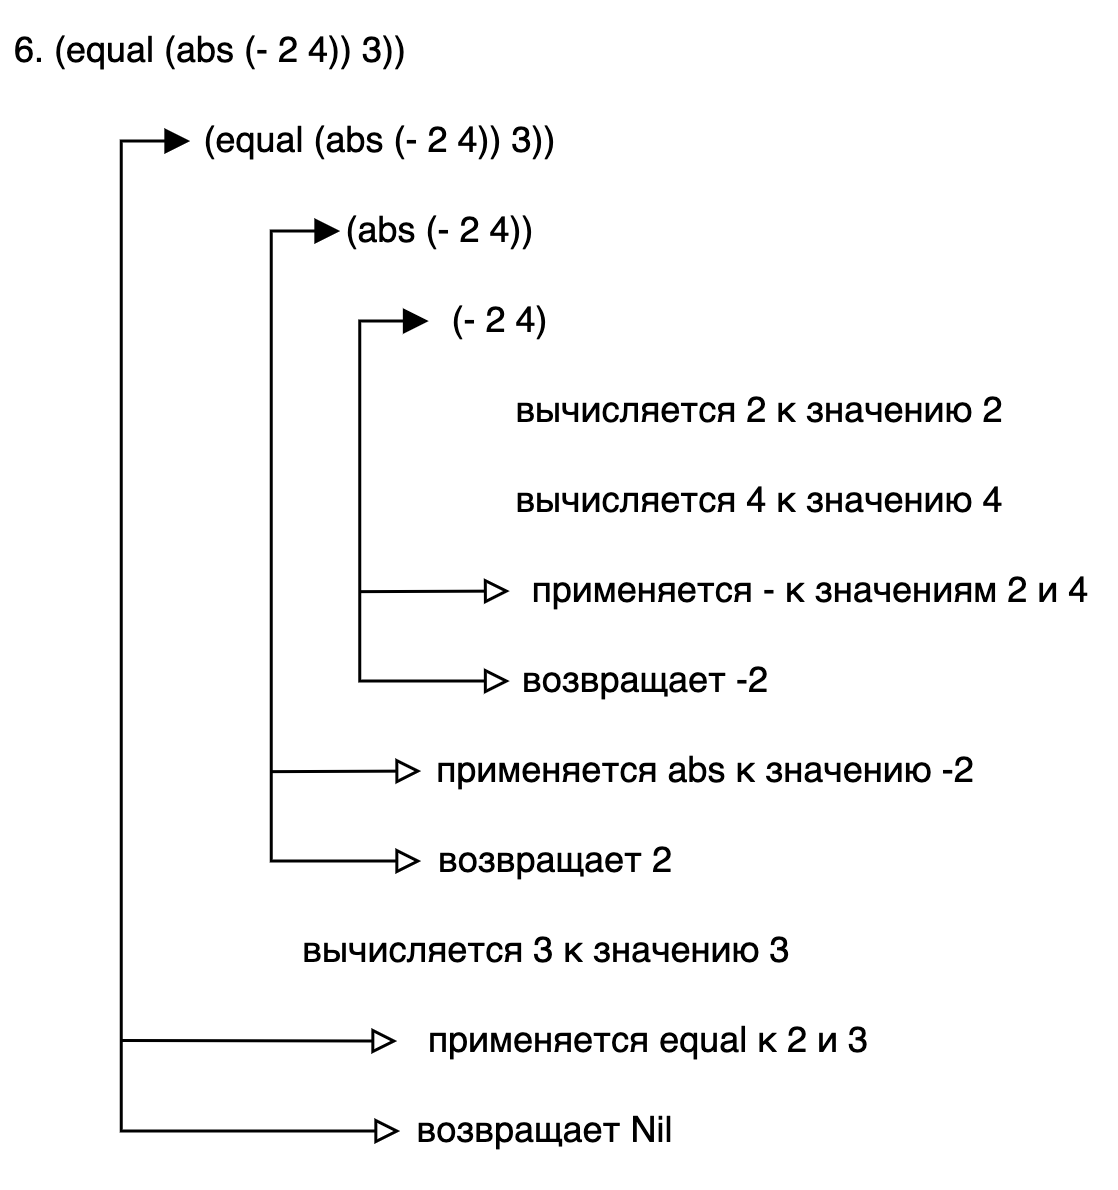
\includegraphics[scale=0.5,left]{task1.6}
\end{figure}
\clearpage

\section*{Задание 2. Написать функцию, вычисляющую гипотенузу прямоугольного треугольника по заданным катетам и составить диаграмму её вычисления.}

\begin{lstinputlisting}[
	caption={Задание 2},
	label={lst:t2},
	style={lsp},
	linerange={3-4},
	]{../src/main.lsp}
\end{lstinputlisting}

\begin{figure}[h!]
	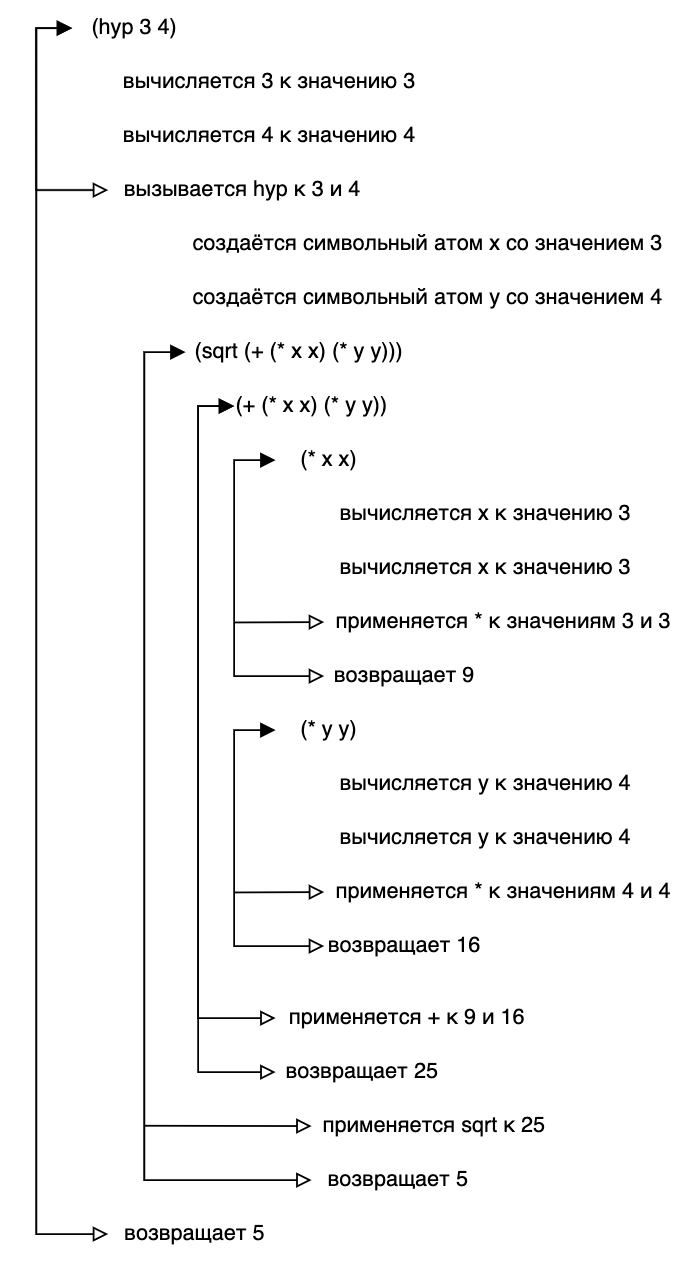
\includegraphics[scale=0.75,left]{task2}
\end{figure}

\section*{Задание 3. Каковы результаты вычисления следующих выражений?(объяснить возможную ошибку и варианты ее устраненения)}

\begin{lstinputlisting}[
	caption={Задание 3},
	label={lst:t3},
	style={lsp},
	linerange={6-13},
	]{../src/main.lsp}
\end{lstinputlisting}

\section*{Задание 4.Написать функцию longer\_then от двух списков-аргументов, которая возвращает Т, если первый аргумент имеет большую длину.}

\begin{lstinputlisting}[
	caption={Задание 4},
	label={lst:t4},
	style={lsp},
	linerange={15-16},
	]{../src/main.lsp}
\end{lstinputlisting}

\section*{Задание 5. Каковы результаты вычисления следующих выражений?}
\clearpage

\begin{lstinputlisting}[
	caption={Задание 5},
	label={lst:t4},
	style={lsp},
	linerange={18-25},
	]{../src/main.lsp}
\end{lstinputlisting}

\section*{Задание 6. Дана функция (defun mystery (x) (list (second x) (first x))). Какие результаты вычисления следующих выражений?}

\begin{lstinputlisting}[
	caption={Задание 6},
	label={lst:t4},
	style={lsp},
	linerange={29-36},
	]{../src/main.lsp}
\end{lstinputlisting}

\section*{Задание 7.Написать функцию, которая переводит температуру в системе Фаренгейта температуру по Цельсию (defum f-to-c (temp)...).}
Формулы:  $c = 5 / 9 * (f - 32.0)$, $f = 9 / 5 * c + 32.0$

\begin{lstinputlisting}[
	caption={Задание 7},
	label={lst:t4},
	style={lsp},
	linerange={38-39},
	]{../src/main.lsp}
\end{lstinputlisting}
Как бы назывался роман Р.Брэдбери "+451 по Фаренгейту" в системе по Цельсию?

Ответ: "232.78 по Цельсию"

\section*{Задание 8. Что получится при вычислении каждого из выражений?}

\begin{lstinputlisting}[
	caption={Задание 7},
	label={lst:t4},
	style={lsp},
	linerange={43-49},
	]{../src/main.lsp}
\end{lstinputlisting}


